% Intro section
\subsection{Deviation from Plan}
	\subsubsection{Development Approach}
		% Organic dev approach
		% Didn't know what processes the app would use
	\subsubsection{Measurement Process}
		\paragraph{Use of EXIF Data and Reference Point}
			% Began trying to use exif data but some stuff couldn't be found
			% Changed to finding ref point which works great
		\paragraph{Dynamic Measurement Limits}
			% Initially using middle third of image
			% Finding the o-ring creates dynamic point
			% Uses finding contours in both methods
			\begin{figure}[h!]
				\centering
				\begin{minipage}{0.4\textwidth}
					\centering
					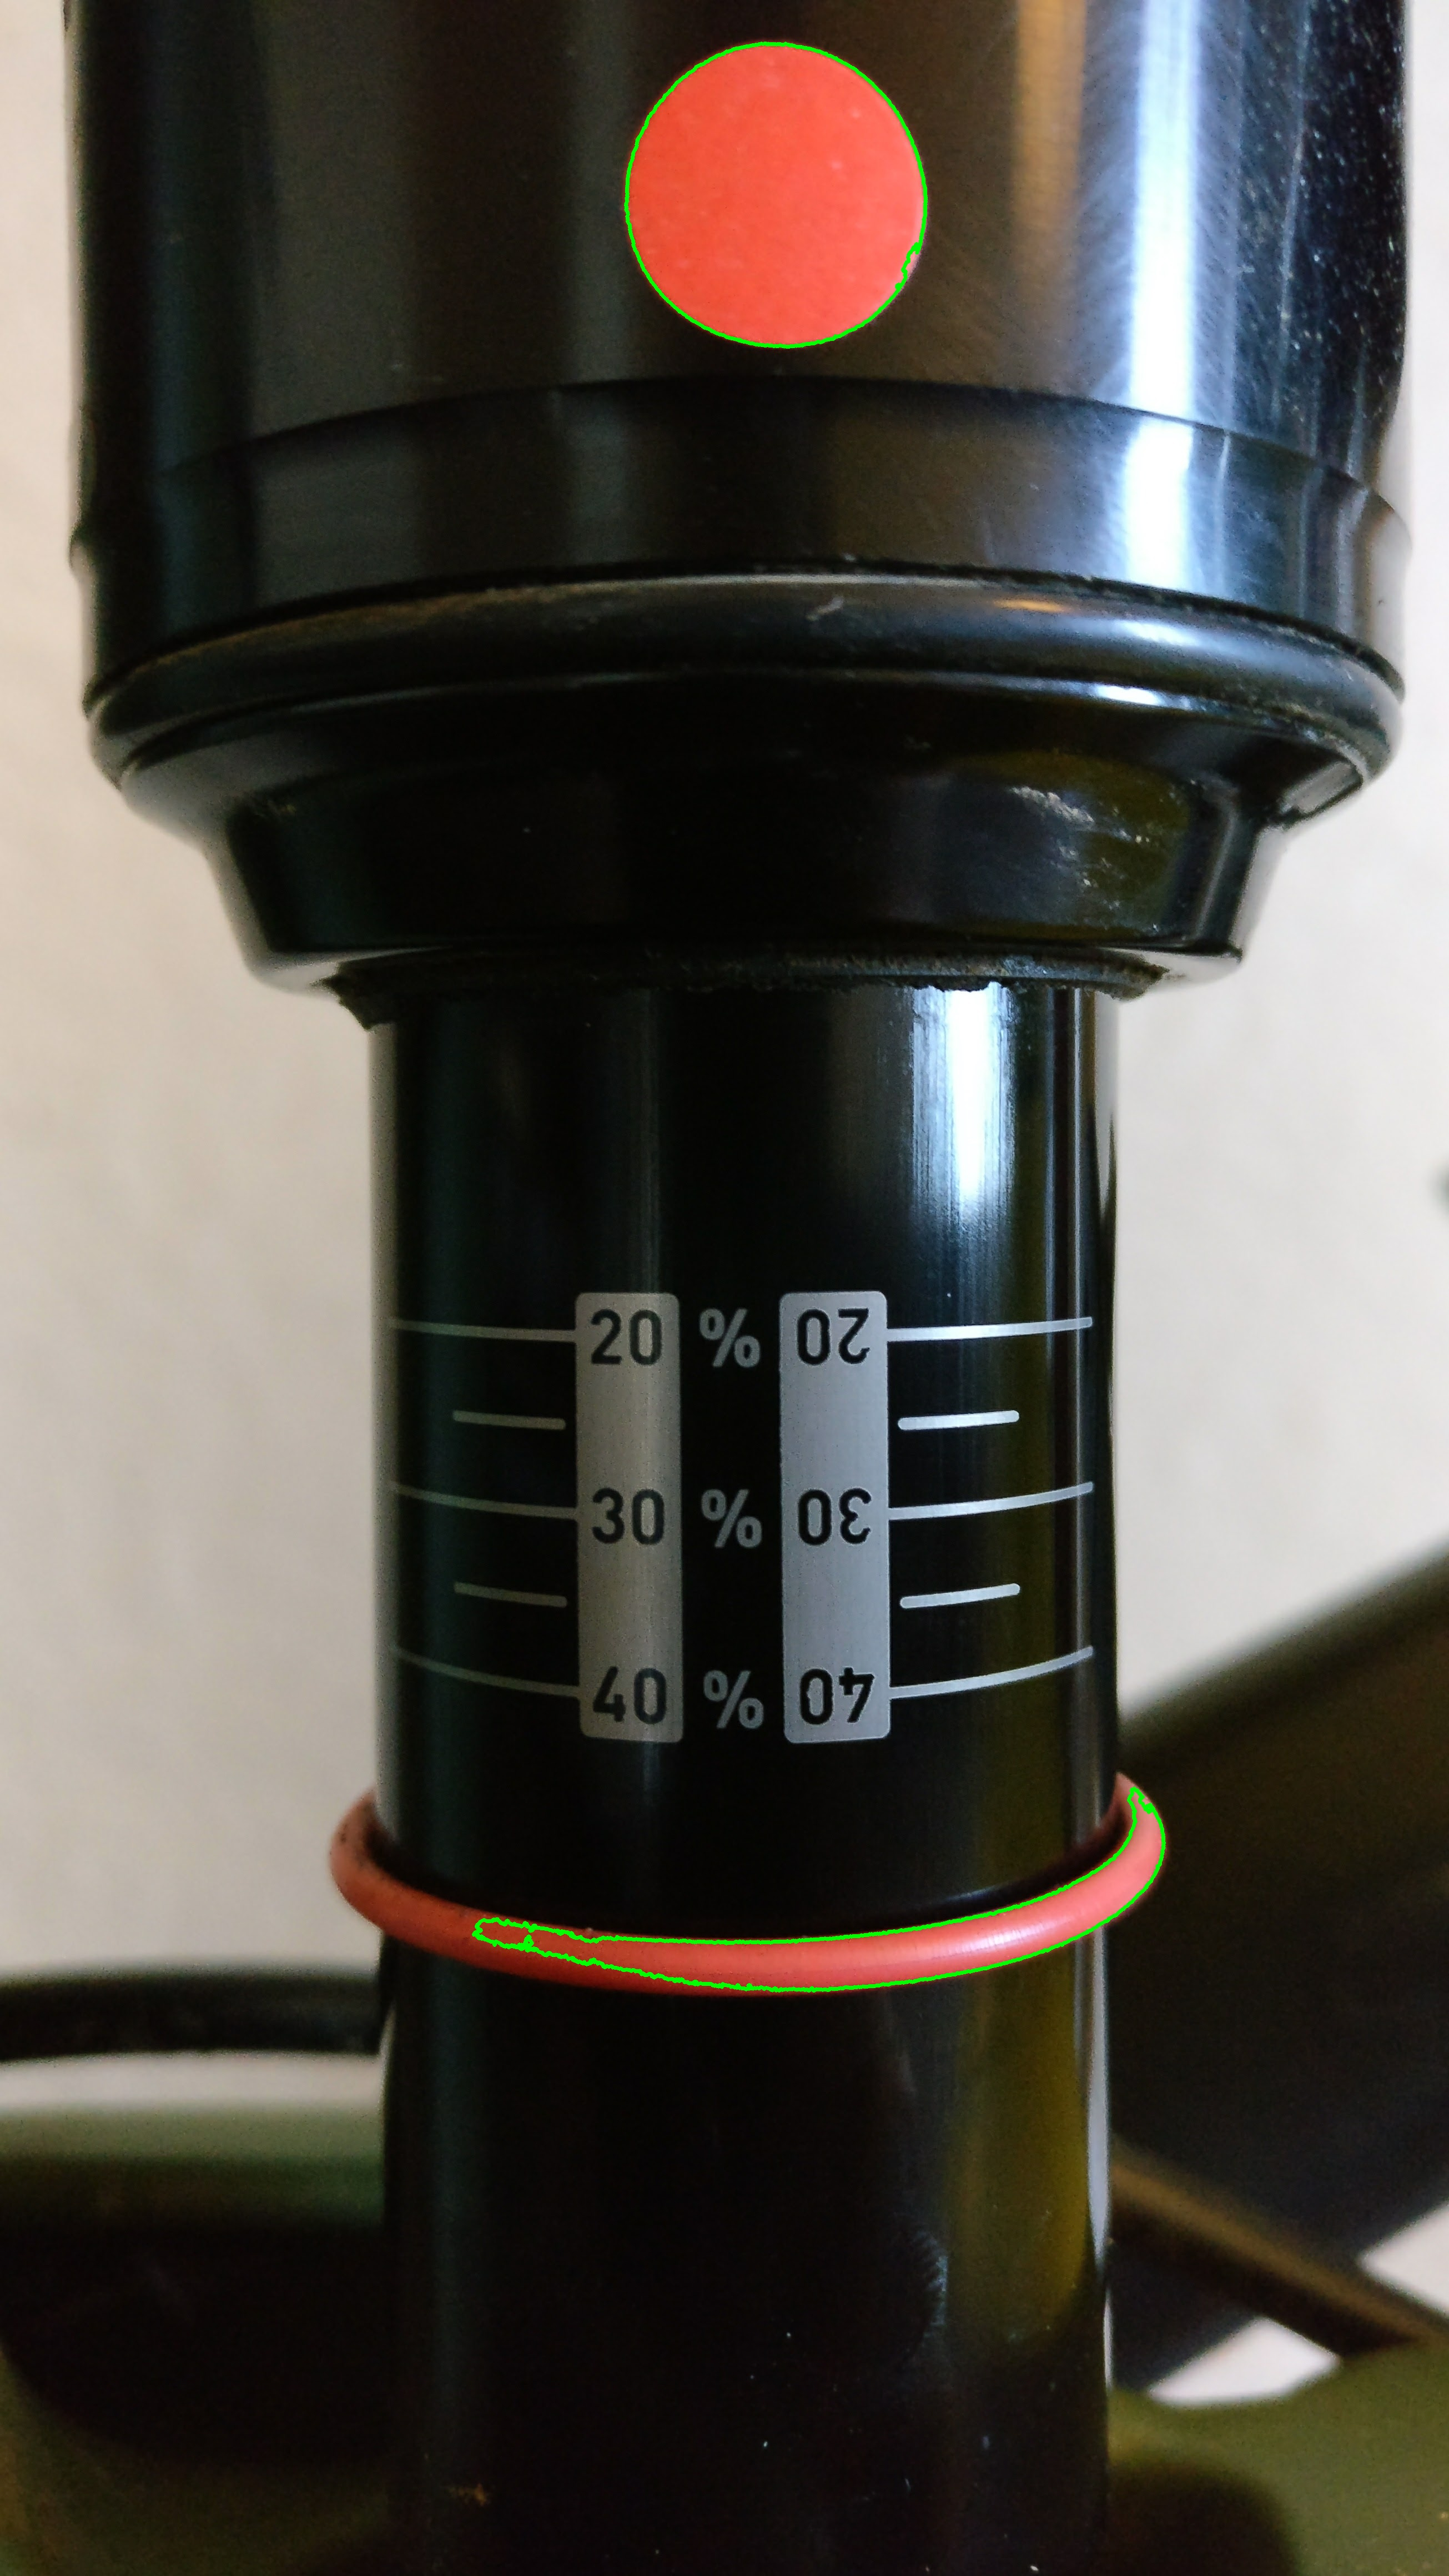
\includegraphics[scale=0.1,
					trim={20cm 30cm 15cm 110cm},
					clip]{../images/results/contours.jpg}				
				\end{minipage}
				\begin{minipage}{0.4\textwidth}
					\centering
					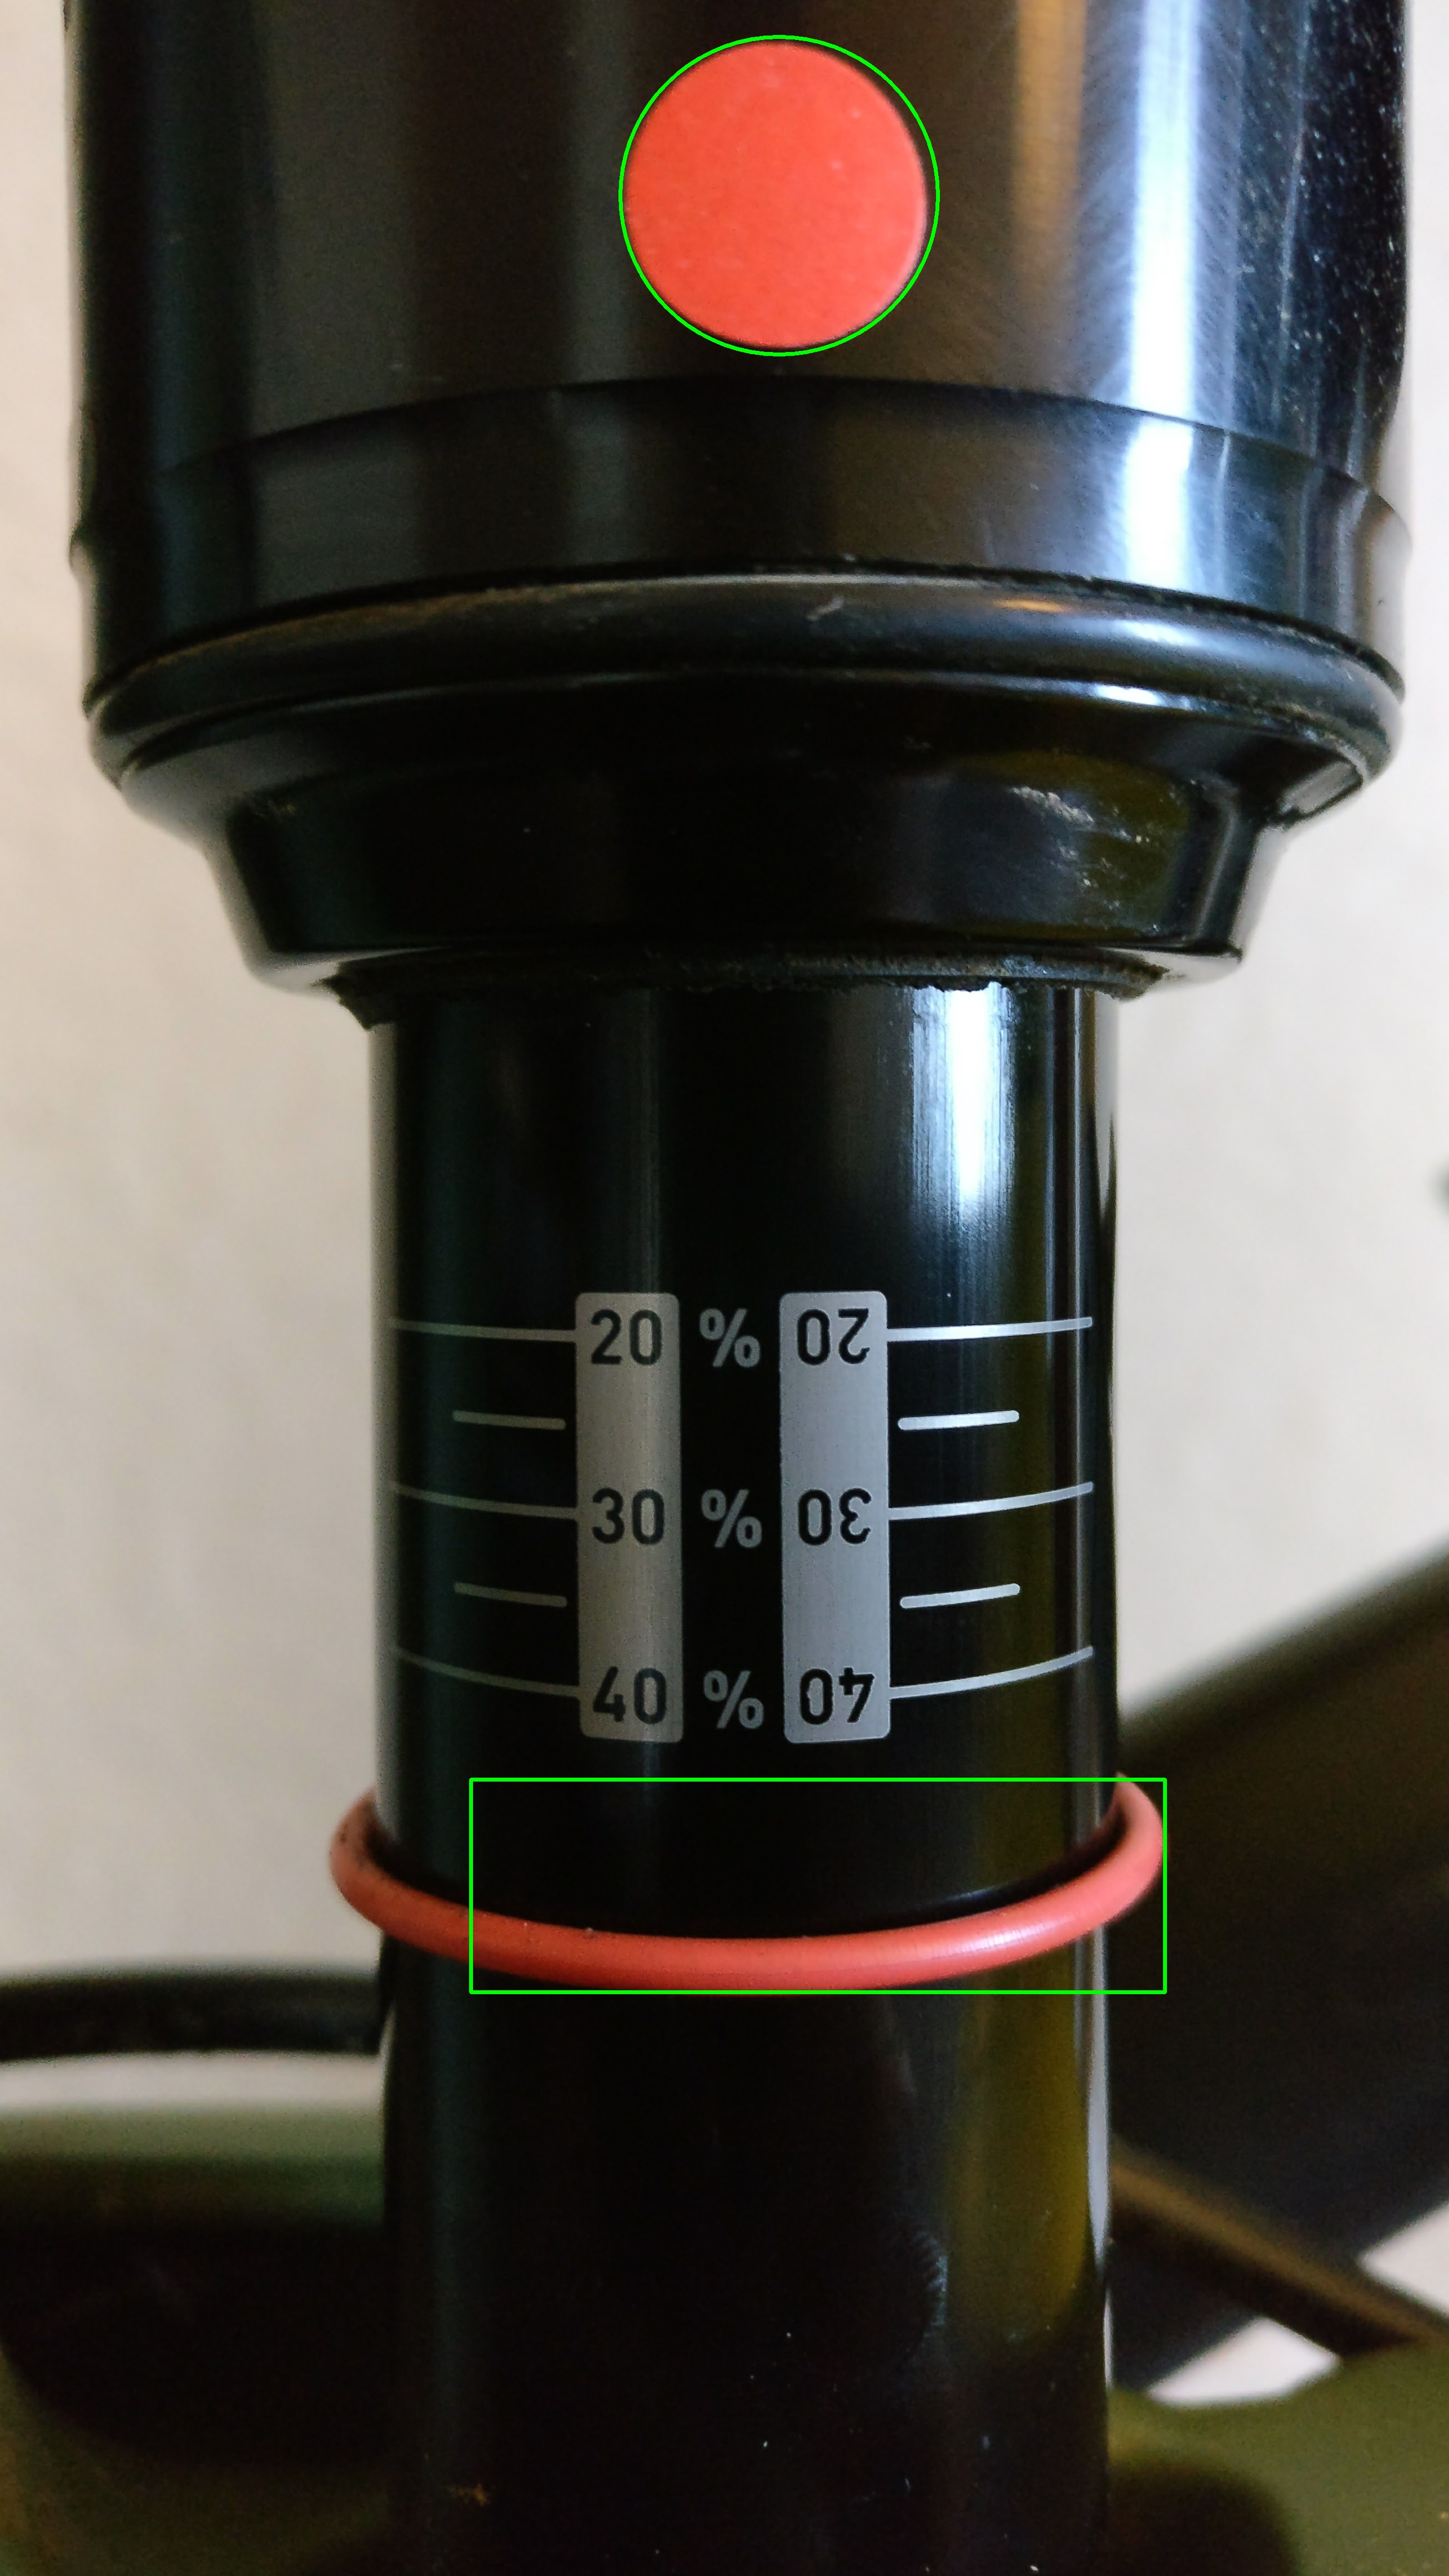
\includegraphics[scale=0.1,
					trim={20cm 30cm 15cm 110cm},
					clip]{../images/results/raw_refs.jpg}				
				\end{minipage}\hfill
				\caption{O-ring found using findContours (left) with boundingBox applied (right)}
				\label{fig:find_oring}
			\end{figure}
		\paragraph{Reference Point Location Method}
			% Hough circles was unreliable
				% Reproduce images
			% Find contours always produces the same result, takes longer
			\begin{figure}[h!]
				\centering
				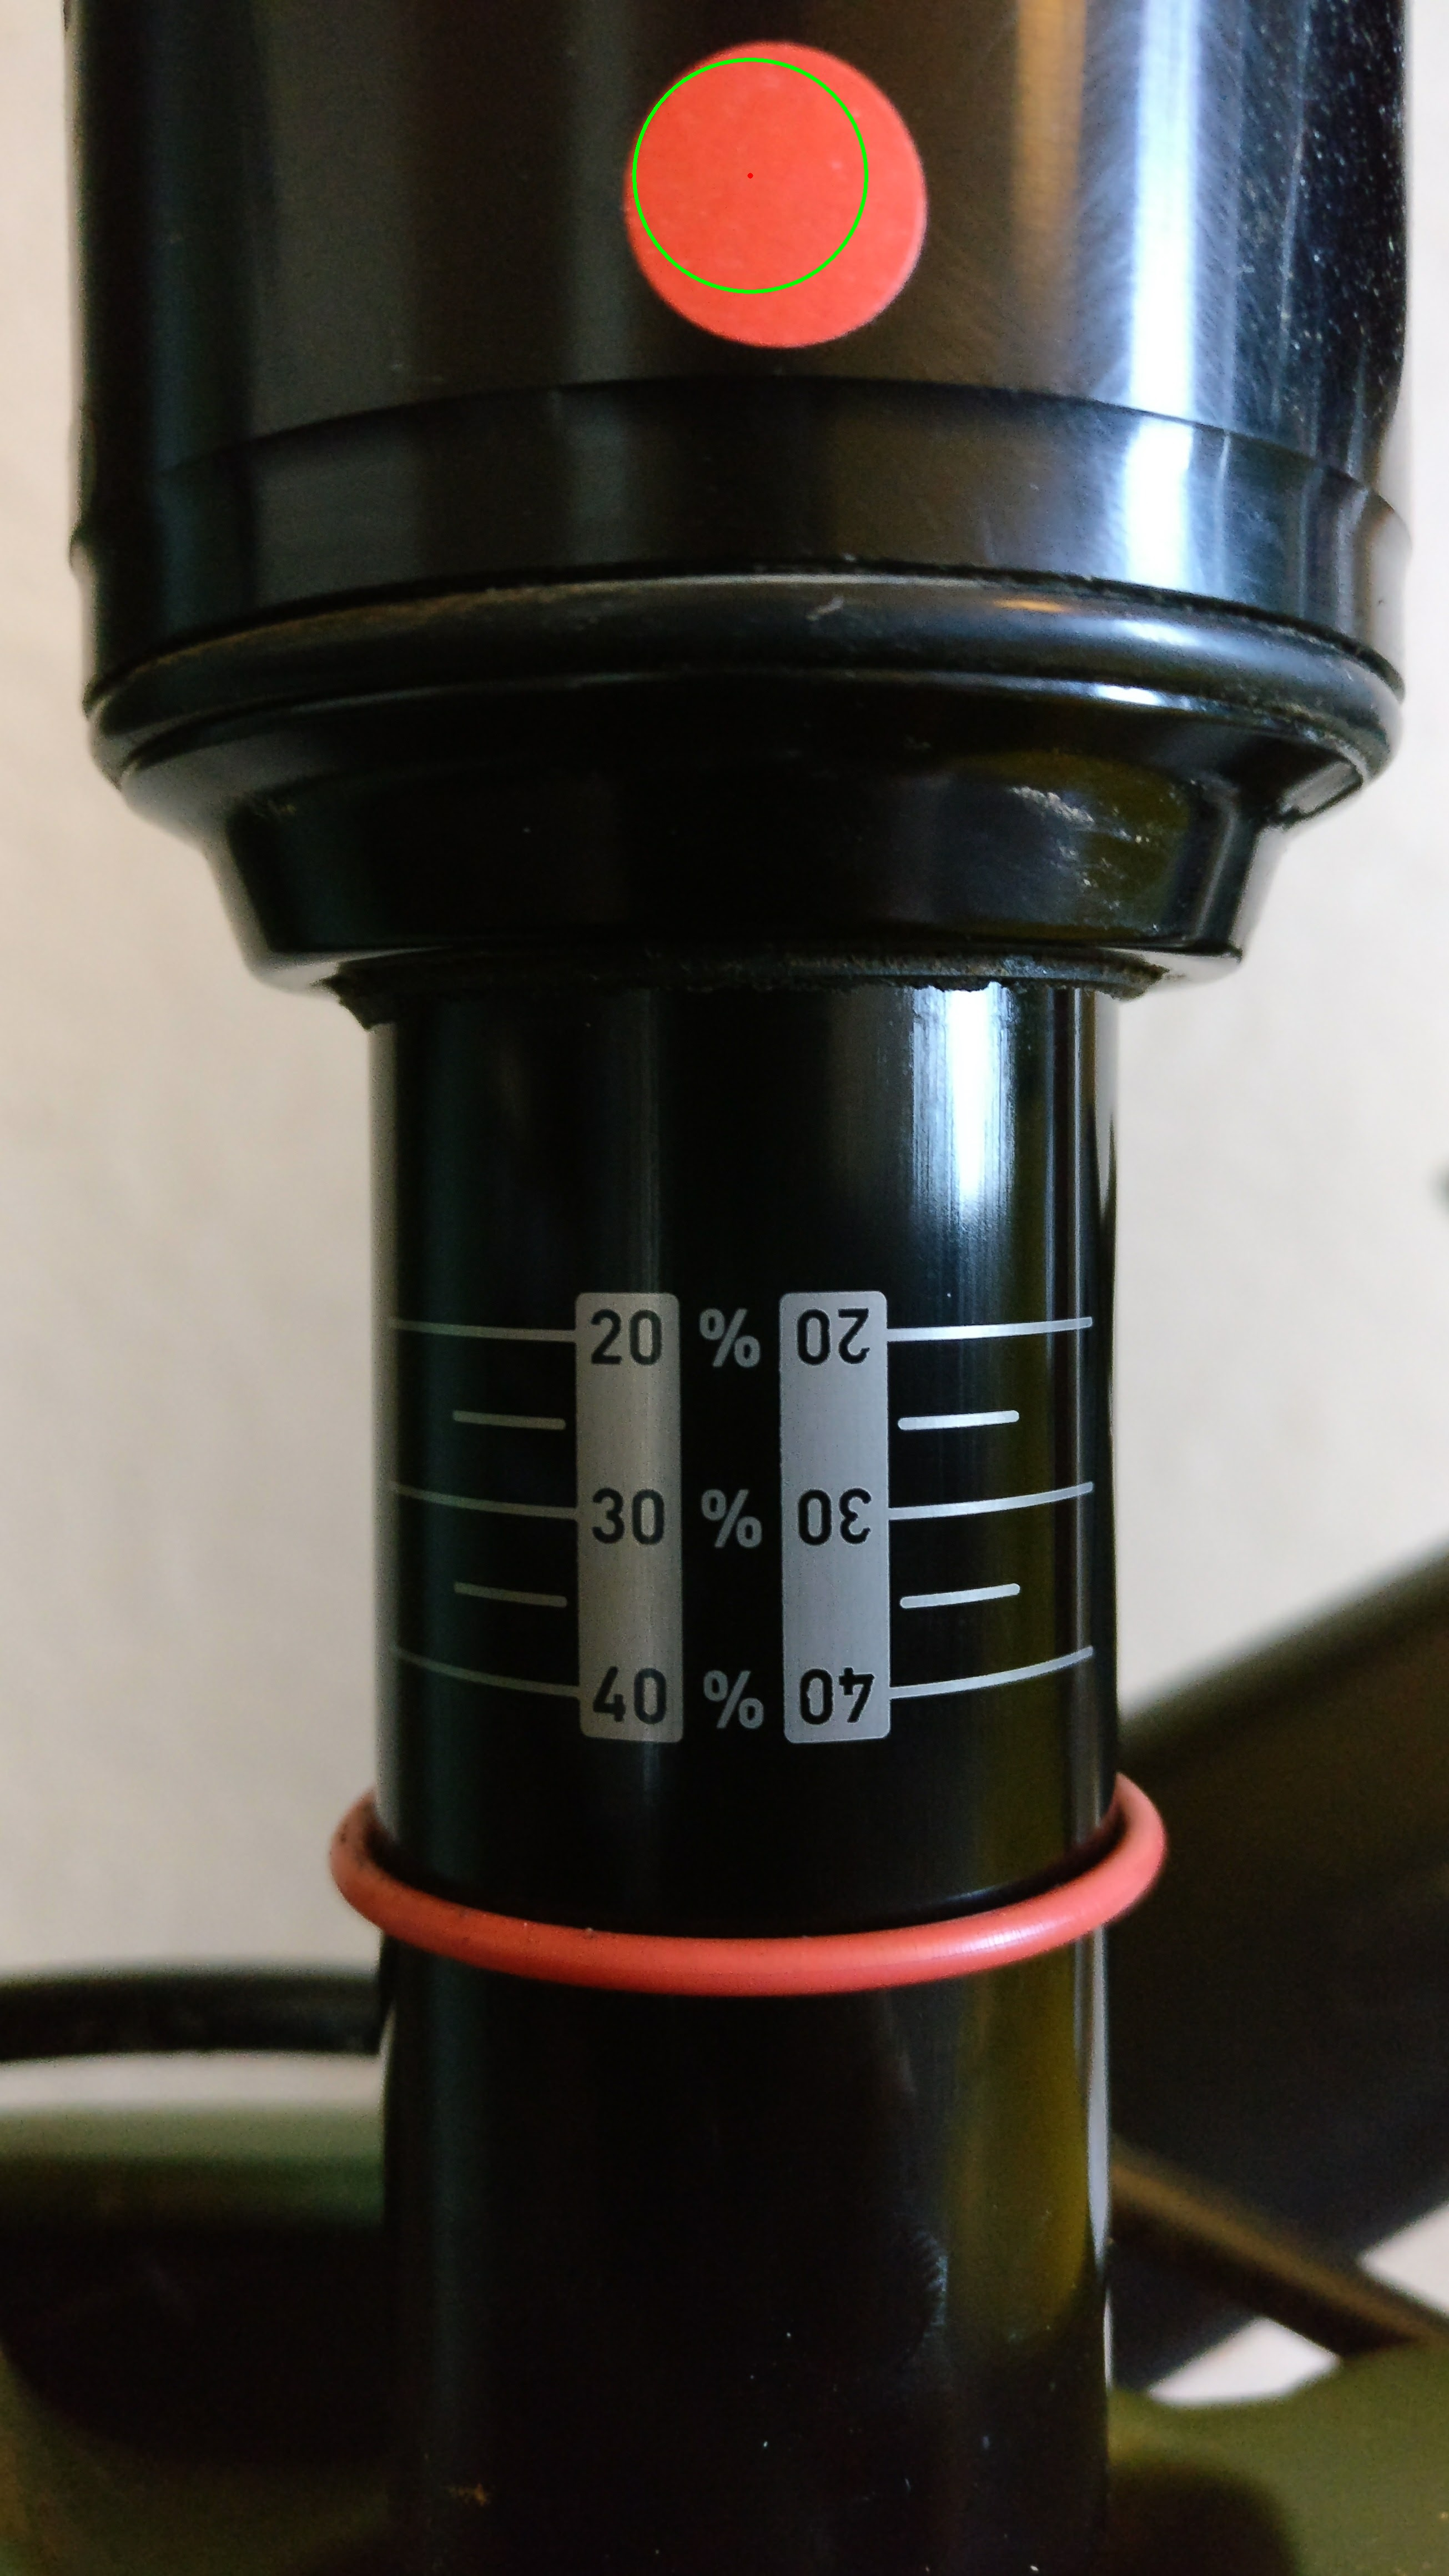
\includegraphics[scale=0.1,
				trim={30cm 140cm 25cm 0},
				clip]{../images/results/HoughCircles.jpg}
				\caption{Reference point found using HoughCircles}
				\label{fig:hough_circle}
			\end{figure}
			\begin{figure}[h!]
				\centering
				\begin{minipage}{0.4\textwidth}
					\centering
					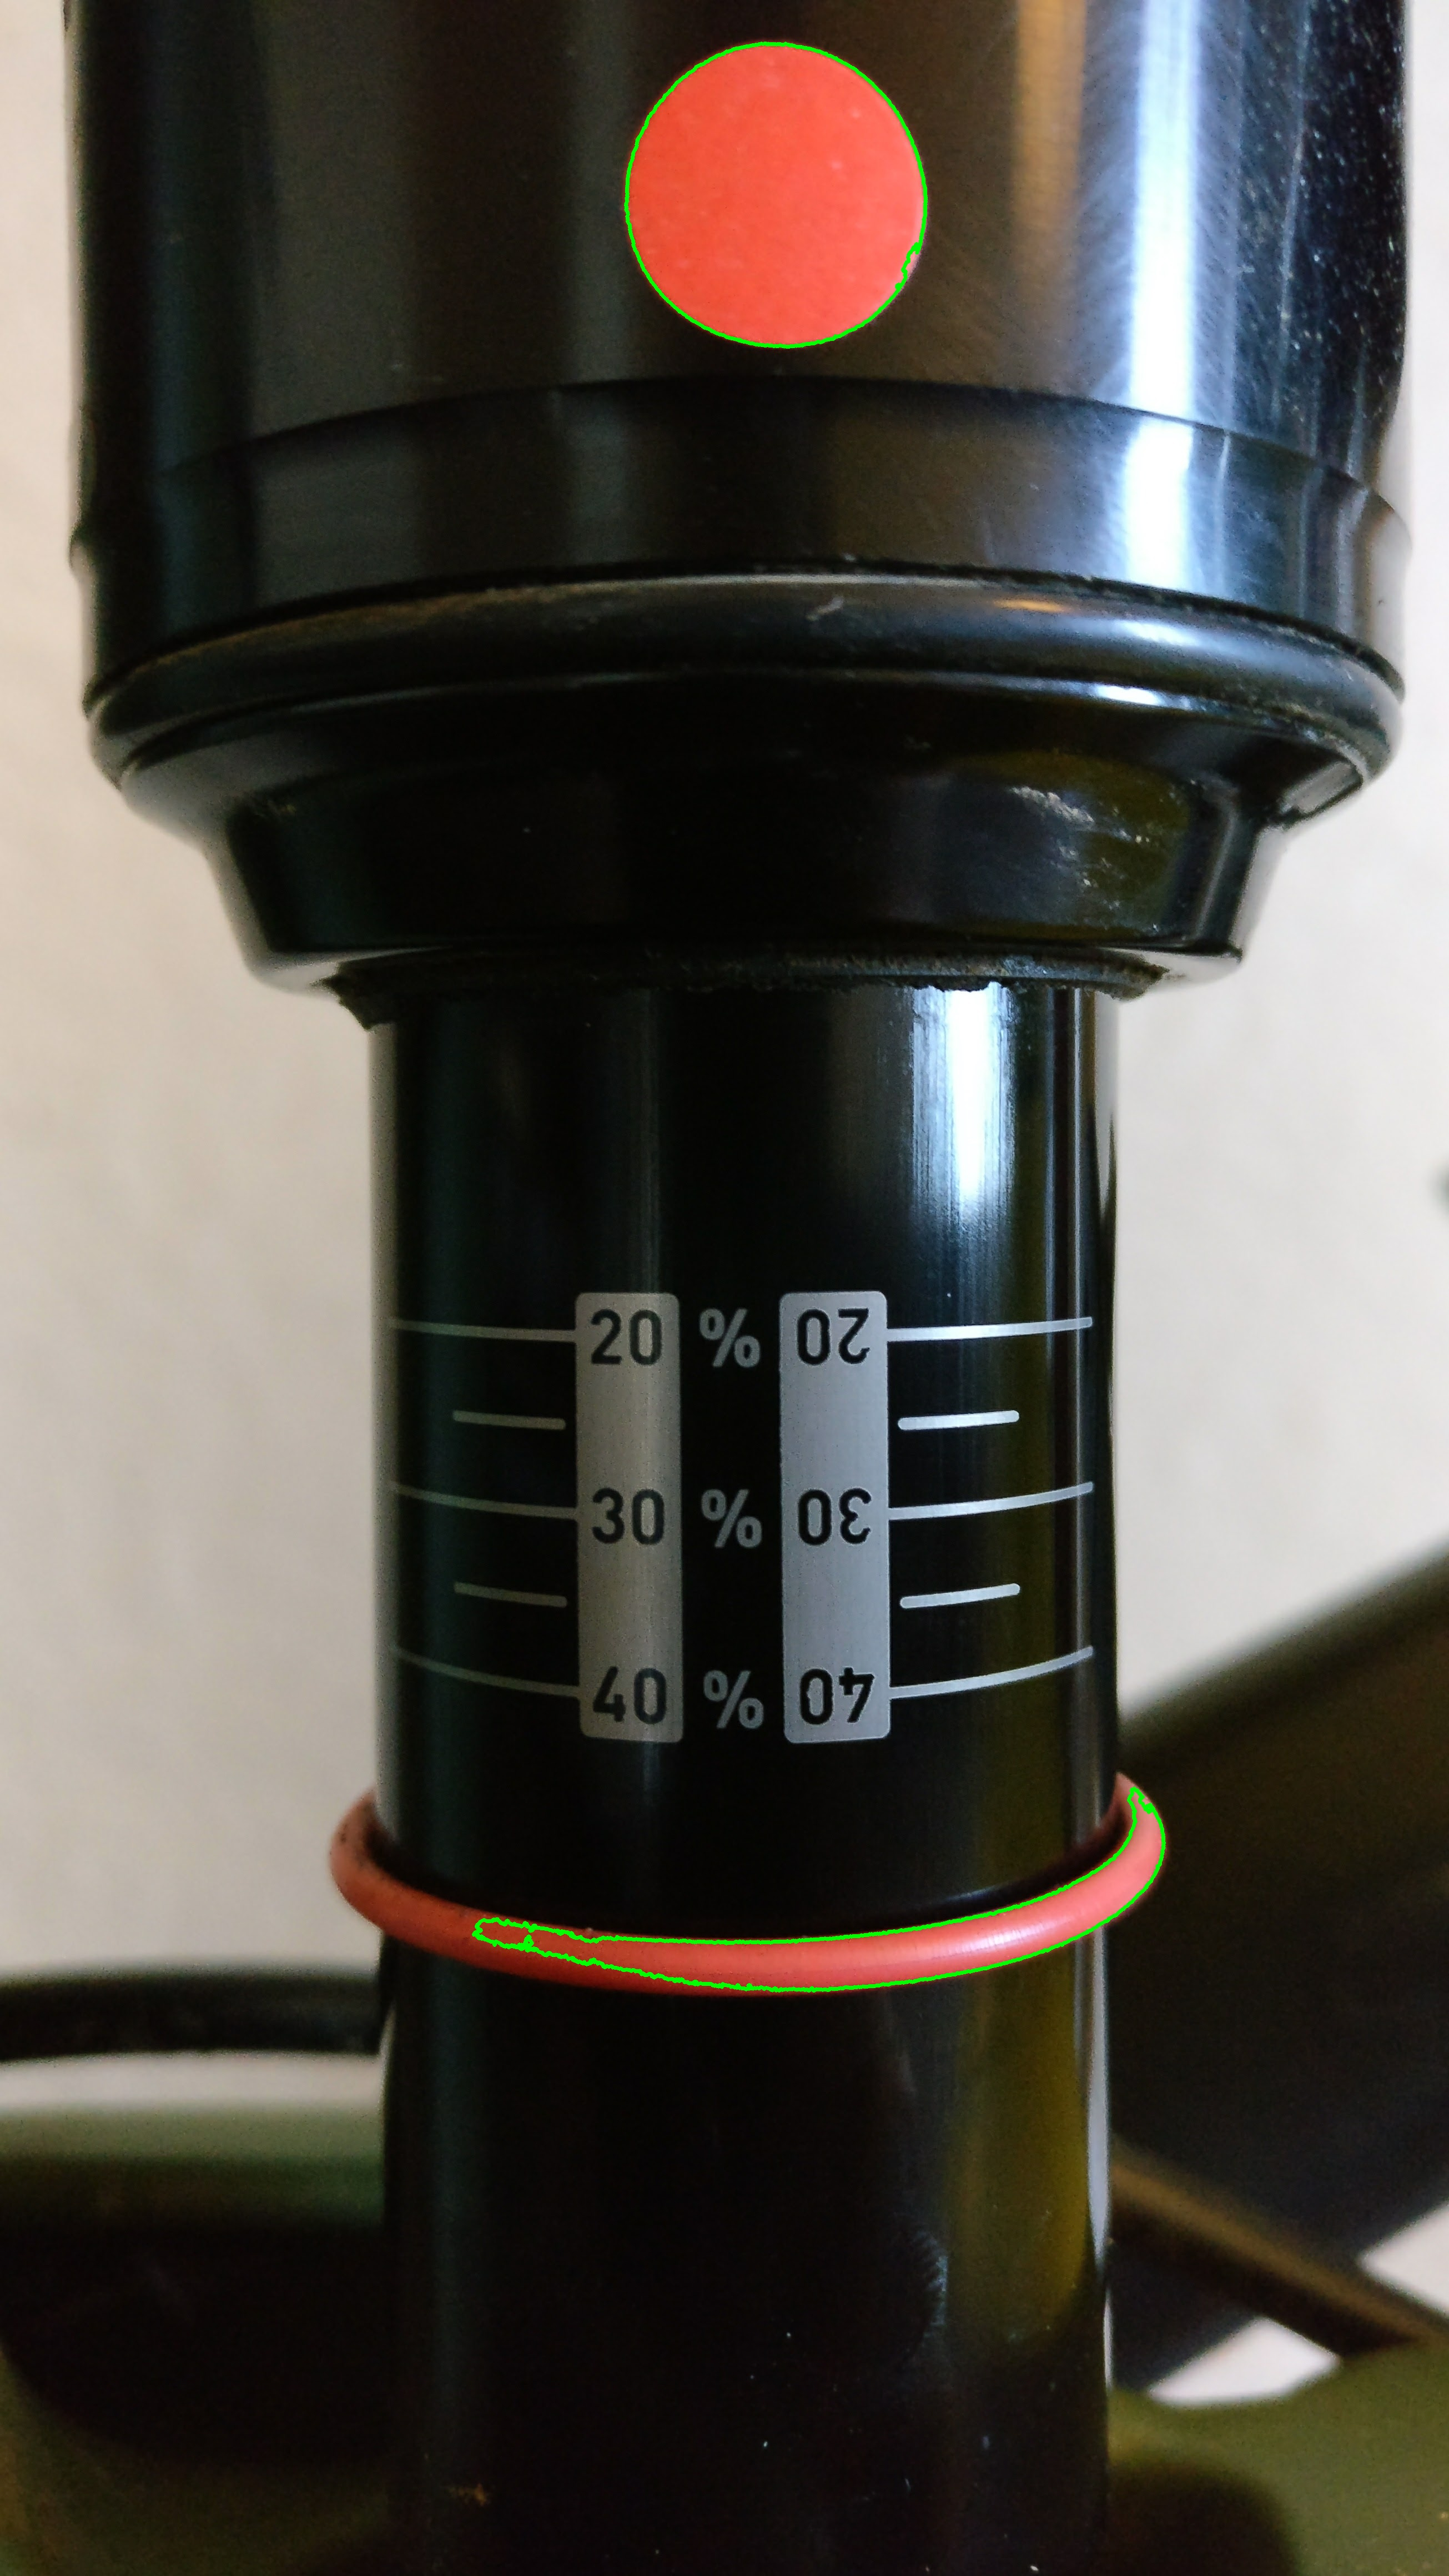
\includegraphics[scale=0.1,
					trim={30cm 140cm 25cm 0},
					clip]{../images/results/contours.jpg}				
				\end{minipage}
				\begin{minipage}{0.4\textwidth}
					\centering
					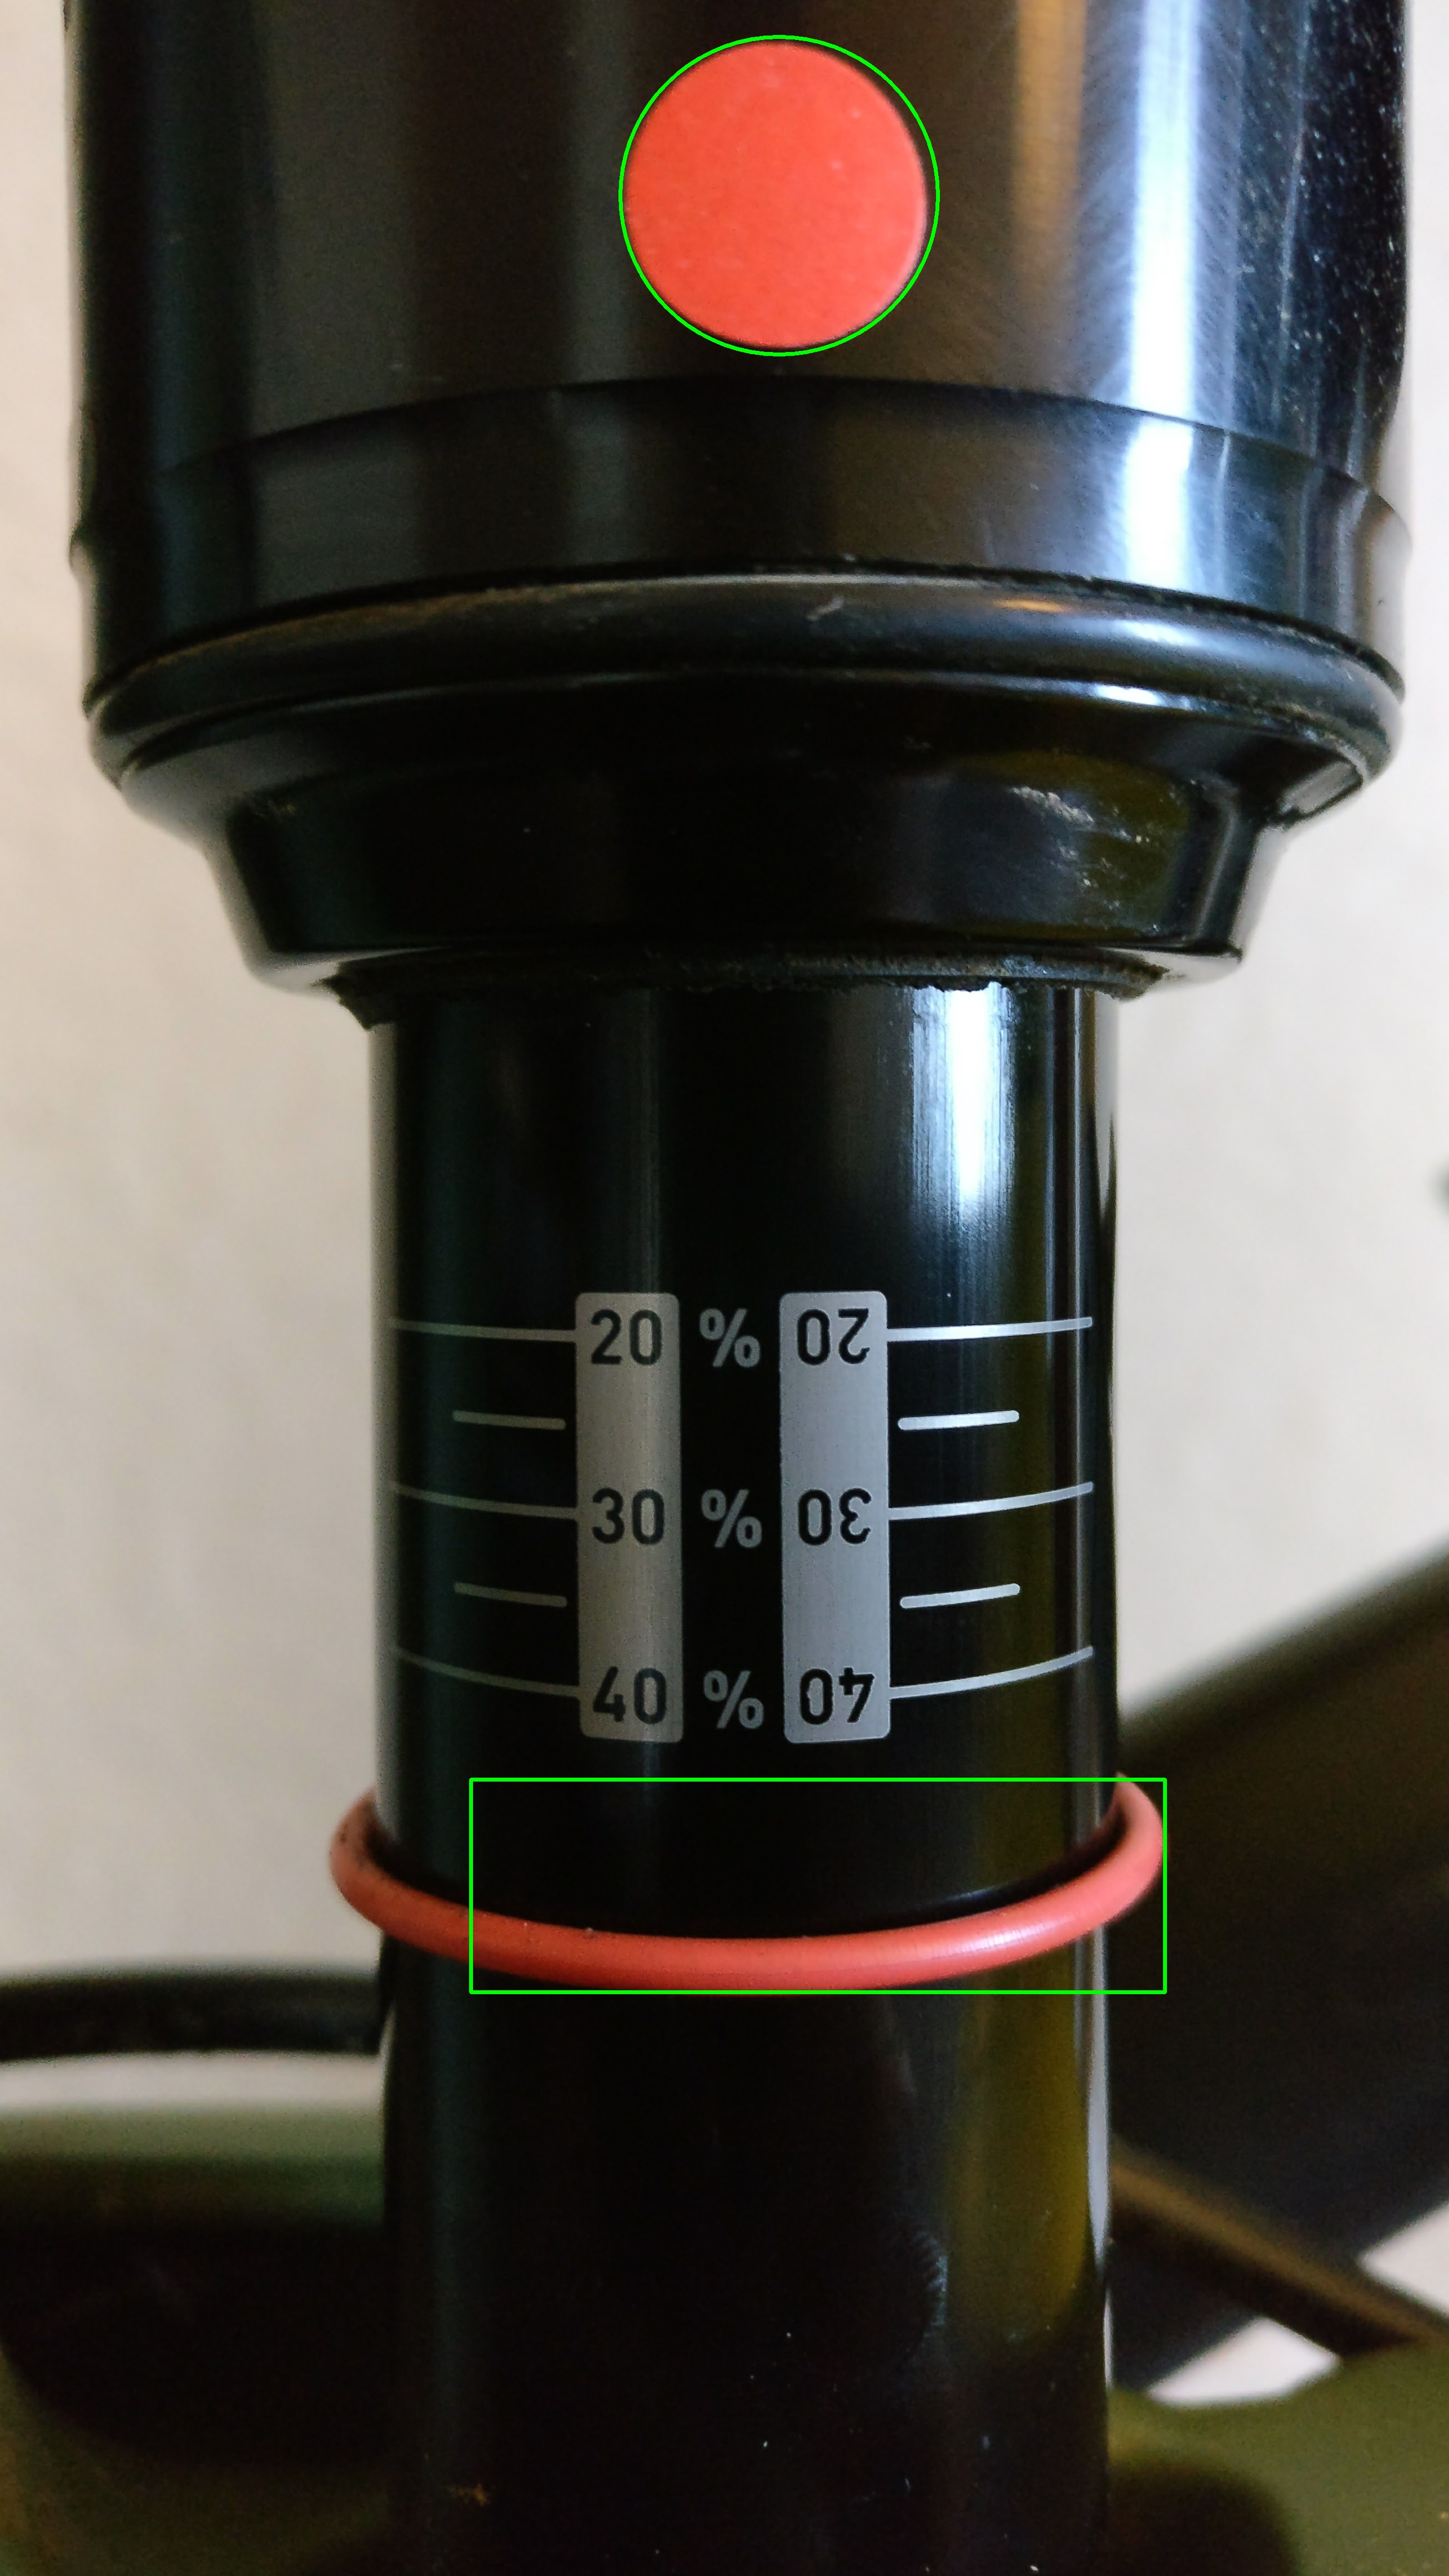
\includegraphics[scale=0.1,
					trim={30cm 140cm 25cm 0},
					clip]{../images/results/raw_refs.jpg}				
				\end{minipage}\hfill
				\caption{Reference point found using findContours (left) with boundingCircle applied (right)}
				\label{fig:find_ref}
			\end{figure}
		\paragraph{Pressure Calculation}
			% Inital idea was psi per mm, doesn't work because of non linerarity
			% Ran experiments to see if it is linear
			% Added dynamic function into app
\subsection{System}
\subsection{Critical Evaluation}
	\subsubsection{Validation}
	\subsubsection{Reliability and Accuracy}
		\begin{table}[h!]
			\centering
			\caption{Table of uncertainty calculation results}
			\label{tab:uncertainty}
		\begin{tabular}{|l|r|r|r|r|}
			\hline
			\multirow{12}{7em}{\bfseries Measurements}&\multicolumn{2}{|l|}{\bfseries Rockshox}&\multicolumn{2}{|l|}{\bfseries Fox}\\
			\cline{2-5}
			&\bfseries 25\%&\bfseries 30\%&\bfseries 25\%&\bfseries 30\%\\
			\hline
			&175.02&160.97&133.31&120.54\\
			&174.84&160.52&133.28&120.47\\
			&174.95&160.41&133.42&120.48\\
			&174.83&160.65&133.42&120.46\\
			&174.94&160.75&133.29&120.53\\
			&174.86&160.50&133.38&120.51\\
			&175.63&160.48&133.35&120.50\\
			&174.78&160.77&133.36&120.46\\
			&175.29&160.57&133.36&120.46\\
			&174.84&160.74&133.42&120.50\\
			\hline
			\bfseries Average&175.00&160.64&133.36&120.49\\
			\bfseries Standard Deviation&0.27&0.17&0.05&0.03\\
			\bfseries Uncertainty&175 $\pm$ 0.27&160.64 $\pm$ 0.17&133.36 $\pm$ 0.05&120.49 $\pm$ 0.03\\
			\hline
		\end{tabular}
		\end{table}
	\subsubsection{Comparison to Alternatives}
	\subsubsection{Professional Opinion}